\documentclass[pageno]{jpaper}

\newcommand{\asplossubmissionnumber}{336}

\usepackage[normalem]{ulem}
\usepackage{booktabs}   % For formal tables: http://ctan.org/pkg/booktabs
\usepackage{subcaption} % For complex figures with subfigures/subcaptions http://ctan.org/pkg/subcaption
\usepackage{soul}
\usepackage{amssymb}
\usepackage{amsmath}
\usepackage{algorithm} % environment for the algorithm code (like figure and table)
\usepackage{algorithmicx} % write the pseudo code
\usepackage[noend]{algpseudocode} % layout of the pseudo code
\usepackage{tikz} % needed for: tikz pics
\usepackage{xcolor}
\usepackage{xspace}
\usepackage{listings}
\usepackage{hyphenat}
\usepackage{wrapfig}
\usepackage{multirow}
\usepackage{capt-of}
\usepackage{siunitx}
\usepackage{flushend}

\hypersetup{colorlinks=false,linkcolor=blue,urlcolor=blue}

%\usepackage[normalem]{ulem}
%\usepackage{float}
%
%\usepackage{titlesec} %P{rzemek: ommented, has conflict https://tex.stackexchange.com/questions/321999/conflict-between-makeuppercase-in-title-formatting-and-usepackagexcolor
%
%\titlespacing{\section}{0pt}{0.5\baselineskip}{\parskip}
%\titlespacing{\subsection}{0pt}{0.5\baselineskip}{\parskip}
%\titlespacing{\subsubsection}{0pt}{0.5\baselineskip}{\parskip}
%\titlespacing{\section}{2pt}{0.8\baselineskip}{\parskip}
%\titlespacing{\subsection}{2pt}{0.6\baselineskip}{\parskip}
%\titlespacing{\subsubsection}{2pt}{0.6\baselineskip}{\parskip}
%
%\setlength{\textfloatsep}{5pt}% Remove \textfloatsep
%
%\usepackage[keeplastbox]{flushend} %Brandon: this broke the build for me
%Added for sub-float package from jpaper.cls - will check later
%\RequirePackage[font={normalsize,sf,bf}]{caption}
%\RequirePackage[position=bottom]{subfig}
%\captionsetup[table]{aboveskip=0.5em, belowskip=0.5em}
%\captionsetup[figure]{aboveskip=0.5em, belowskip=0em}
%\captionsetup[subfloat]{font={small,sf}}
%
\newlength{\sectionbelowskip}
\newlength{\sectionaboveskip}
\newlength{\subsectionbelowskip}
\newlength{\subsectionaboveskip}
\newlength{\paragraphaboveskip}
%
% Defaults in sigplanconf (note that horizontal space after \paragraph heading will be different):
%\setlength{\sectionbelowskip}{4pt}
%\setlength{\sectionaboveskip}{10pt plus 3pt minus 2pt}
%\setlength{\subsectionbelowskip}{4pt}
%\setlength{\subsectionaboveskip}{8pt plus 2pt minus 2pt}
%\setlength{\paragraphaboveskip}{6pt plus 2pt minus 2pt}
%
% Slightly tighter than defaults:
% \setlength{\sectionbelowskip}{3pt}
% \setlength{\sectionaboveskip}{6pt plus 2pt minus 2pt}
% \setlength{\subsectionbelowskip}{2pt}
% \setlength{\subsectionaboveskip}{4pt plus 1pt minus 1pt}
% \setlength{\paragraphaboveskip}{2pt plus 1pt minus 1pt}
%
\algnewcommand{\LeftComment}[2][.5\linewidth]{%
  \leavevmode\makebox[#1][l]{$\triangleright$~#2}\hfill}

% Tighter than defaults:
%\setlength{\sectionbelowskip}{1pt}
\setlength{\sectionbelowskip}{4pt}
\setlength{\sectionaboveskip}{5pt plus 1.5pt minus 1.5pt}
\setlength{\subsectionbelowskip}{1pt}
\setlength{\subsectionaboveskip}{3pt plus 1pt minus 1pt}
\setlength{\paragraphaboveskip}{1pt plus 1pt minus 1pt}
%
\newcommand{\TODO}[1]{{\bf \em \textcolor{red}{TODO: #1}\xspace}}
\newcommand{\todo}[2]{\textcolor{red}{$\bullet$ \textbf{Task:} #1; \textbf{Responsible:} #2}}
\newcommand{\note}[1]{\textcolor{red}{[#1]}}
\newcommand{\add}[1]{\textcolor{blue}{#1}}
\newcommand{\remove}[1]{\textcolor{red}{\st{#1}}}
\newcommand{\replace}[2]{\remove{#1} \add{#2}}
\newcommand{\transition}{{\tt coala\_next\_task}\xspace}
\newcommand{\sys}{Coala}

\newcommand{\sysfull}{Dynamic Task-Based Intermittent Execution for Energy-Harvesting Devices}
% \newcommand{\sysmed}{\sys: Adaptive Task-Based Intermittent Execution}
% \newcommand{\sysfull}{\sys: Adaptive Task-Based Intermittent Execution}
%\newcommand{\sysmed}{\sys: Adaptive Intermittent Execution Model$\ldots$}
% \newcommand{\sysmed}{\sys: Adaptive Task-Based Intermittent Execution Model for Energy-harvesting Devices}
%\newcommand{\sysmed}{\sys: Adaptive Task Coalescing for Intermittent Computing $\ldots$}
%\newcommand{\sysfull}{\sys: Adaptive Task Coalescing for Intermittent Computing on Energy-harvesting Devices}
%newcommand{\sysfull}{\sys: Efficient Task-based Intermittent Computing with Adaptive Task Coalescing and Memory Virtualization} %Old title

\begin{document}

\title{\sysfull}         %% [Short Title] is optional;
\date{}
\maketitle
%
%% when present, will be used in
%% header instead of Full Title.
%\titlenote{}             %% \titlenote is optional;
%% can be repeated if necessary;
%% contents suppressed with 'anonymous'
%\subtitle{}                     %% \subtitle is optional
%\subtitlenote{}       %% \subtitlenote is optional;
%% can be repeated if necessary;
%% contents suppressed with 'anonymous'
%
%Note: order of authors placed randomly
%
% \author{Kiwan Maeng}
% \authornote{}
% \orcid{}
% \affiliation{%
% 	\institution{Carnegie Mellon University}
% 	\streetaddress{4720 Forbes Avenue}
%    \city{Pittsburgh} 
% 	\state{PA} 
% 	\postcode{15213}
% }
% \email{kmaeng@andrew.cmu.edu}
%
% \author{Alexei Colin}
% \authornote{}
% \orcid{}
% \affiliation{%
% 	\institution{Carnegie Mellon University}
% 	\streetaddress{4720 Forbes Avenue}
% 	\city{Pittsburgh} 
% 	\state{PA} 
% 	\postcode{15213}
% }
% \email{acolin@andrew.cmu.edu}
%
% \author{Carlo Delle Donne}
% \authornote{}
% \orcid{}
% \affiliation{%
% 	\institution{Delft University of Technology}
% 	\streetaddress{Van Mourik Broekmanweg 6}
% 	\city{Delft, The Netherlands} 
% 	\state{Zuid Holland} 
% 	\postcode{2628\,XE}
% }
% \email{c.delledonne@student.tudelft.nl}
%
% \author{Amjad Yousef Majid}
% \authornote{}
% \orcid{}
% \affiliation{%
% 	\institution{Delft University of Technology}
% 	\streetaddress{Van Mourik Broekmanweg 6}
% 	\city{Delft, The Netherlands} 
% 	\state{Zuid Holland} 
% 	\postcode{2628\,XE}
% }
% \email{a.y.majid@tudelft.nl}
%
% \author{Kas{\i}m Sinan Y{\i}ld{\i}r{\i}m}
% \authornote{}
% \orcid{}
% \affiliation{%
% 	\institution{Delft University of Technology}
% 	\streetaddress{Van Mourik Broekmanweg 6}
% 	\city{Delft, The Netherlands} 
% 	\state{Zuid Holland} 
% 	\postcode{2628\,XE}
% }
% \email{k.s.yildirim@tudelft.nl}
%
% \author{Brandon Lucia}
% \authornote{}
% \orcid{}
% \affiliation{%
% 	\institution{Carnegie Mellon University}
% 	\streetaddress{4720 Forbes Avenue}
% 	\city{Pittsburgh} 
% 	\state{PA} 
% 	\postcode{15213}
% }
% \email{blucia@andrew.cmu.edu}
%
% \author{Przemys{\l}aw Pawe{\l}czak}
% \authornote{}
% \orcid{}
% \affiliation{%
% 	\institution{Delft University of Technology}
% 	\streetaddress{Van Mourik Broekmanweg 6}
% 	\city{Delft, The Netherlands} 
% 	\state{Zuid Holland} 
% 	\postcode{2628\,XE}
% }
% \email{p.pawelczak@tudelft.nl}
%
% \renewcommand{\shortauthors}{A. Y. Majid et al.}

\begin{abstract}	
% Connecting the work to a real-world problem
Embedded devices in the Internet of Things (IoT) gain new deployment
opportunities when their hardware is free of batteries and powered by ambient
energy.
% The main problem that we are tackling
Energy harvested from the environment, however, is unpredictable
and can only power a device intermittently.
% The already proposed solution to the main problem
In the intermittent execution model, computation is frequently interrupted by
power failures, and to make forward progress, the system must save intermediate
program state into non-volatile memory.

% The problem of the proposed solutions 
Task-based programming models that execute at the granularity of
statically-defined tasks, offer an efficient alternative to checkpointing.
%
Existing task-based systems, however, fix their task size at compile time and
operate without any regard to the changing energy conditions at runtime.
%
When tasks are sized without accounting for available energy, state may be
persisted either more frequently than unnecessary or not frequently enough for
the program to make progress and terminate.
%
% Our main claim 
To address this challenge, we propose Coala, an \emph{adaptive} task-based
execution model that colesces or downscales static tasks at runtime in response
to changing energy availability.
% show off
% main benefits of Coala
Coala ensures that power failures cannot leave the program state in
non-volatile memory inconsistent using a specialized memory virtualization
mechanism.
%
Our evaluation on a real energy-harvesting device demonstrates the benefits of
adaptive task coalescing and downscaling, and highlights Coala's performance
improvements over a state-of-art task-based system.



\end{abstract}

\section{Introduction}
\label{sec:intro}

Advances in processor efficiency along with the development of energy-harvesting systems have created a new category of devices that require neither a battery nor a tethered power supply~\cite{prasad_comst_2014,lucia_snapl_2017,soyata_csm_2016}. These devices operate using ambient energy, such as radio frequency transmissions~\cite{rf_powered_computing_gollakota_2014},
light~\cite{margolies_infocom_2016,margolies_tosn_2016}, and vibration~\cite{gorlatova_sigmetrics_2014}. Incorporating compute, storage, sensing, and communication hardware~\cite{wisp5,moo,capybara}, such devices are a promising technology for use in the Internet of Things~\cite{ku_cst_2016}, in-body~\cite{nadeau_naturebio_2017} and on-body~\cite{bandodkar_electroanalysis_2015} medical systems, and energy-harvesting nano-satellites~\cite{kicksat,capybara}. Energy-harvesting devices create unique challenges because they operate {\em intermittently} when energy is available~\cite{hicks_isca_2017,lucia_snapl_2017}. An energy-harvesting device buffers energy in a small storage capacitor~\cite{gorlatova_tmc_2013,gunduz_commag_2014} and operates when a threshold amount of energy has accumulated. Harvestable energy sources are low-power (e.g., \si{\nano\watt}\ to \si{\micro\watt}) compared to a platform's operating power level (hundreds of \si{\micro\watt}\ to \si{\milli\watt}). A device operates briefly until it depletes its buffered energy, after which, it shuts down and recharges to operate again later---corresponding to the {\em intermittent execution model}~\cite{dino,lucia_snapl_2017} composed of operation---power failure---restart cycles. The recharge and discharge intervals---which correspond to the device's inactive and active time---vary depending on the underlying hardware, such as the size of the energy buffering~\cite{capybara}, and energy conditions. For example, some devices discharge and restart $\approx$10 to $\approx$100 times per second~\cite{tan_infocom_2016,mementos,nvp}.

Upon power failures, a device loses the volatile state in its registers, stack, SRAM, and retains the state of any non-volatile memory, such as FRAM. While capturing periodic checkpoints~\cite{mementos,quickrecall} and sleep scheduling~\cite{dewdrop,hibernus,hibernusplusplus} help preserve execution progress, failures can leave non-volatile state incorrect, partially updated. These inconsistencies cause intermittent execution to deviate from continuously-powered behavior, often leading to an unrecoverable application failure~\cite{dino,edb}. Prior work developed two main approaches to deal with data inconsistency for intermittently-powered devices: (i) \emph{software-based programming and execution models}~\cite{dino,ratchet,chain,alpaca} and (ii) \emph{hardware-based computer architecture support}~\cite{hicks_isca_2017,idetic,nvp}. Complex hardware architectural changes are expensive to design, verify, and manufacture. New hardware architectures are also inapplicable to existing systems~\cite{hicks_isca_2017,nvp}. Software approaches are simpler and applicable to existing devices today. Therefore, this work focuses on software approaches. In particular we address the key limitation of task-based programming and execution model, that is the {\em inflexibility} and \emph{energy-unawareness} of statically decomposing a program into tasks.
%
\begin{figure}
    \centering
    \includegraphics[width=\columnwidth]{figures/intro-figure.pdf}
    \caption{Task coalescing at runtime reduces time and energy overhead in task-based intermittent programming models by performing fewer commits (denoted as \texttt{C}) of individual tasks (denoted as \texttt{Tx}). On the other hand, task splitting reduces wasted computation and enables termination for bigger tasks.}
    \label{fig:coalesce}
\end{figure}

%\textbf{Task Decomposition of Intermittent Programs.} 

\textbf{Crucial Drawback of Static Task Decomposition.} Task-based programming and execution models require a programmer~\cite{alpaca,chain} or a compiler~\cite{baghsorkhi_cgo_2018} to statically decompose a program into a collection of tasks. A \emph{task}, a top level function, can include arbitrary computation that should be executed despite arbitrarily-timed power failures. The programmer (or a compiler) explicitly expresses task-to-task control flow. Fig.~\ref{fig:coalesce} (left) illustrates how a program's tasks execute and shows how tasks transitions can impose a runtime overhead. At each transition, the system incurs an overhead to track and atomically commit modifications to the non-volatile memory, to maintain consistency of program state~\cite{chain,alpaca}. The more task transitions a program requires, the more commit overhead is incurred by the system at runtime. A programmer may thus create very large tasks in an attempt to reduce task transitions overhead. However, a large task may require more energy to complete than a device's fixed hardware energy buffer can hold, which may lead to a task \emph{non-termination} problem (see Fig.~\ref{fig:coalesce}(right)). To eliminate this risk, existing systems require the programmer to decompose a program into small tasks to preserve execution progress. These constraints on task sizing lead to the following \emph{dilemma}: should large tasks be used, that are efficient but risk non-termination, or small tasks that are guaranteed to complete but incur a high task transition and commit overhead?

\textbf{Challenges and Contributions.} We introduce \sys: a new task-based system that employs \emph{adaptive task size execution by task coalescing and splitting}. By means of this novel technique, small tasks can be executed efficiently by trimming unnecessary overheads \emph{dynamically}, meanwhile avoiding the risk of non-termination. \sys accepts any static decomposition and it coalesces (groups) tasks or splits them (see again Fig.~\ref{fig:coalesce}) based on the estimated energy availability without demanding any hardware support. To the best of our knowledge, \sys is the only system that guarantees forward progress for any statically-defined tasks or energy storage sizes. 

The unique contributions of \sys in relation to challenges of task-based systems revealed by this work are as follows:

\begin{itemize}

\item[C1] \emph{Overcoming Task Transition Overhead:} given unpredictable incoming energy, how to save computation state at task transitions as rare as possible? \sys tries to minimize task transition overhead by estimating energy conditions at run-time using \emph{recent execution history} as a metric.

\item[C2] \emph{Dynamic Memory Consistency Handling:} merging static tasks on the fly rises  the need for dynamic memory consistency handling. This leads to the second challenge: how to dynamically detect inter-coalesced-task data dependencies and ensure efficient protection against power interrupts? \sys addresses this challenge by using a novel approach called \emph{dynamic group privatization}---performing real-time dependency tracking to enable protection on a task transition. Individual variables tracking, however, slows down a system dramatically. Therefore, \sys keeps memory consistent through \emph{memory virtualization} optimized for bulk accesses to task-shared data with high locality.

%Therefore, \sys protects global variables in a batch. Moreover, it optimizes data transfers by using Direct Memory Access (DMA).

\item[C3] \emph{Ensuring Task Termination:} a static task decomposition model assumes that each task can execute to completion. If the hardware energy buffer provides inadequate energy to execute each task to completion, a program will not terminate~\cite{cleancut_2018}. This leads to a third challenge: how to enable the dynamic execution model to progress on a sub-task level? To avoid non-termination under adverse energy conditions, \sys uses a novel timer-based {\em partial task commit} mechanism, inspired by~\cite{ratchet}. Partial execution avoids non-termination by committing the intermediate state of a long-running task that has repeatedly failed and restarted.

\end{itemize}

To asses the benefits of \sys over existing task-based systems, we implemented and tested six benchmarks on a real energy-harvesting platform. Our evaluation not only shows that \sys reduces run time by up to 54\%, and by 26\% on average, but also is able to continue the execution where static task-based systems fail.
 
The rest of this paper is organized as follows. Section~\ref{sec:background} provides background on intermittent computing.
Section~\ref{sec:systemdescription} provides an overview of \sys, while Section~\ref{sec:task_adaptation} describes \sys's task adaptation mechanism. The dynamic group privatization is explained in Section~\ref{sec:memory_virtulaization}. Implementation details of \sys are given in Section~\ref{sec:implementation}. Sections~\ref{sec:methodology} and~\ref{sec:evaluation} describe \sys's evaluation methodology and results. Section~\ref{sec:related_work} positions \sys in the context of related work and Section~\ref{sec:conclusions} concludes and discusses future work.

% \clearpage % hack to get rid of rophan
\section{Intermittent Computing: Background}
\label{sec:background}

In this section, we provide background on energy harvesting systems and the intermittent software execution model. We then discuss the key limitations of existing task-based execution models for intermittent computing that \sys
addresses.

\subsection{Energy Harvesting Systems}
\label{sec:background_harvesting}

Energy harvesting devices operate using energy extracted from their environment, from sources such as radio waves (RF) and solar energy. Energy-harvesting devices need not use a tethered power supply or battery and instead, typically collect energy into a (super-)capacitor, operate when sufficient energy has accumulated, and upon depleting the stored energy, turn off and wait to collect more energy.

Batteryless operation has a number of important advantages, making intermittent computing an important research domain. Supplying power to billions~\cite{gartner_iot} of embedded computers using batteries is not sustainable. The European Commission estimates that more than 160 kilotons of consumer batteries enter the European Union annually~\cite{eu_batteries_2016}. Batteries are an environmental risk, are fragile, are limited in their number of charge/discharge cycles, and may require costly physical maintenance that is difficult or impossible deployed (e.g. in space~\cite{kicksat}). By contrast, super-capacitors are durable, promising millions of charge/discharge cycles~\cite[Sec. I]{ongaro_pwre_2012}. The main limitation in moving to capacitor-based energy storage is that capacitor energy density---and consequently operating discharge time---is orders of magnitude less than a battery. 

%Given current technology development, battery-less systems are best suited for very long-term sensing and monitoring where access to recharge is either prohibitive or impossible. These include battery-less image capture and processing~\cite{naderiparizi_rfid_2015}, animal monitoring~\cite{thomas_jbcs_2012} or implantable~\cite{rodriguez_tbcs_2015} and digestible~\cite{nadeau_naturebio_2017} sensors.

Many platforms enable intermittent, battery-less computation. For instance, computation RFIDs---open-source TI MSP430-based~\cite{wolverine} WISP~\cite{wisp5} (with its variants such as WISPCam~\cite{naderiparizi_rfid_2015}, NFC-WISP~\cite{zhao_rfid_2015} or NeuralWISP~\cite{holleman_biocas_2008}), Moo~\cite{moo}, and commercial ones such as~\cite{medusa_farsens_2017}. Other intermittently-powered platforms include ambient backscatter tag~\cite{liu_sigcomm_2013,parks_sigcomm_2014} or battery-less phone~\cite{talla_imwut_2017}. In all of the above, the main source of energy harvested is the electromagnetic radiation in the radio frequency range (ambient transmitters such as high power TV transmitters~\cite{liu_sigcomm_2013} or dedicated RFID antenna~\cite{wisp5,moo,talla_imwut_2017,medusa_farsens_2017,holleman_biocas_2008,naderiparizi_rfid_2015}). Naturally, other forms of energy harvesting sources exist, including temperature gradient, (micro-)motions, light/sun radiation, vibrations, and body fluid flow (blood, gastric acid). Several recent surveys discussing energy harvesting, low-power, embedded systems and intermittent computing at a high level~\cite{paradiso_pvc_2005,soyata_csm_2016,prasad_comst_2014,ku_cst_2016,lucia_snapl_2017}.

\begin{table}
	\centering
	\footnotesize
	\begin{tabular}{|c|c|}
		\hline
		Platform name & Storage capacitor size \\
		\hline \hline
		Moo~\cite{moo} & 0.1\,F \\
		WISPCam~\cite{naderiparizi_rfid_2015} & 6.08\,mF \\ %tested [11.24, 17.45, 21.98]\,mF
		NFC-WISP~\cite{zhao_rfid_2015} & 300\,$\mu$F \\
		NeuralWISP~\cite{holleman_biocas_2008} & 100\,$\mu$F \\
		WISP~\cite{wisp5} & 47\,$\mu$F \\
		{\em BioImpedance} sensor~\cite{rodriguez_tbcs_2015} & 20\,$\mu$F \\
		{\em Ingestible} sensor~\cite{nadeau_naturebio_2017} & 220\,$\mu$F\\
		\hline
	\end{tabular} 
	\caption{Comparison of {\em default} energy storage sizes for various battery-less platforms. Observe a huge variation in storage capacity. We note that values for other representative platforms~\cite{medusa_farsens_2017,talla_imwut_2017,liu_sigcomm_2013,parks_sigcomm_2014} were not reported in their respective papers.}
	\label{table:capacitor}
\end{table}

\subsection{Intermittent Computing}
\label{sec:background_consistency}
Energy-harvesting devices execute software according to the {\em intermittent
execution model}~\cite{dino,chain,alpaca,ratchet}.  Physically, a device
charges until a threshold, operates briefly until its energy is depleted, shuts
down recharges, and repeats the cycle.  Software running on the device executes
{\em intermittently} because energy is only available between when the
capacitor reaches its threshold and when it is depleted. An intermittent
execution is composed of operating periods interspersed with power failures.
The frequency of power failures in an intermittent execution depends on the
size of the device's energy storage buffer: a larger buffer allows longer
operating periods.  Energy-harvesters provide input power that is orders of
magnitude less than a device's operating power, making recharging negligible
during operation.

Software has different behavior when executed intermittently than when executed
with continuous power.  Each power failure clears volatile memory (registers,
stack, and global variables). Non-volatile memory (e.g., FRAM) persists across
power failures. On a power failure, control flows back to a prior point in the
execution. By default, after a power failure control flows to the beginning of
{\tt main()}. Early work on intermittent computing preserve intermittent
progress by periodically capturing and restoring to a non-volatile checkpoint
of the volatile execution context (i.e., registers and
stack)~\cite{mementos,hibernusplusplus,quickrecall,idetic}

\begin{figure}
	\centering
	\subfloat[Simplified C code snippet of a CRC calculation from~\cite{hicks_mibench2_2016}: per-byte message division by a polynomial; \texttt{NV} denotes non-volatile variable declaration]{\includegraphics[width=\columnwidth]{figures/crc_example}\label{fig:crc_example}}\\
	\subfloat[Consecutive execution steps of the loop body in the snippet above: non-volatile checkpointing did not guarantee data consistency as data has been manipulated (line 10) with stale reminder (line 3)]{\includegraphics[width=\columnwidth]{figures/crc_example_war}\label{fig:crc_example_war}}
	\caption{Code example demonstrating effect of write after read on volatile memory checkpointing.}
	\label{fig:code_demo_incosistency}
\end{figure}

Checkpoints of volatile state preserve intermittent progress, but do not ensure
data consistency~\cite{dino,chain,ratchet}.  Data may become inconsistent if an
attempt to execute some computation {\em writes} to a non-volatile variable,
then power fails, then a second attempt to re-execute the same computation
incorrectly {\em reads} the value written in the first attempt, rather than the
variable's original value.  The situation occurs when code includes a write
after read (WAR) dependence between operations that manipulate non-volatile
variables~\cite{ratchet,dino,alpaca}.

Figure~\ref{fig:code_demo_incosistency} illustrates how state can become
inconsistent in an intermittent execution using cyclic redundancy check (CRC)
code from MIBench~\cite{hicks_mibench2_2016}. The code computes CRC for an
$\texttt{nBytes}$ byte message $\texttt{msg}$ with remainder $\texttt{Rmnd}$.
Even with the checkpoint at line 3 in Fig.~\ref{fig:crc_example}, the code may
compute  $\texttt{data}$ incorrectly because  of a WAR dependence between the
read of $\texttt{Rmnd}$ on line 4 and the write of $\texttt{Rmnd}$ on line 5.  
Figure~\ref{fig:crc_example_war} shows an execution of the code in which
power fails during the second loop iteration

 $\texttt{Rmnd}$ is read (line 6 in Fig.~\ref{fig:crc_example_war}), or more
specifically---updated before a new execution loop. 

As the figure illustrates, checkpoint-based systems risk violating the
consistency of volatile and non-volatile memory~\cite{dino}. To maintain memory
consistency, versioning systems~\cite{dino,ratchet} {\em version} a subset of
non-volatile variables with the checkpointed execution context. Task-based
systems~\cite{chain,alpaca}, which we focus on this work and discuss in detail
next, ensure state is consistent by using programmer, compiler, and runtime
support.


\subsection{Task-based Intermittent Computing}
\label{section:background_task_computing}

%\TODO{This sequential/modular split seems pretty odd to me. I think we can just talk about tasks in the sense of ratchet, alpaca, and chain.  Anything with static (programmer-written or compiler inserted) boundaries applies}

Intermittent execution models combatting WAR can be classified into: \emph{sequential execution model} (which historically formed a baseline for this stream of research) and \emph{modular execution model} (a potent alternative, on which we base the design decisions of \sys). \todo{Remove division per sequential/modular split}{Przemek}

Under this model a program for intermittently-powered device is seen as a one idempotent operational region with one common context. Generally, the progress of the program is saved and updated by means of checkpointing, refer again to Section~\ref{sec:background_consistency}. Normally, the sequential model relies on a hardware assistant to measure the voltage level in the energy reservoir to place a checkpoint~\cite{mementos,mottola2017harvos,hibernus}. The benefit of this model is that it does not require code modification by a programmer. However it suffers from significant overhead (refer to experiment result in~\cite[Fig. 3]{chain}, where it is concluded that each checkpoint causes overhead). \todo{I use the word `checkpoint' for normal checkpoint and task boundary interchangeably---check if it does not cause confusion}{Brandon}

At the heart of this model is the concept of an \emph{idempotent task}. The idempotent task is a C language function that does not have arguments and does not return a value. This task uses a well defined interface to interact with the non-volatile memory. Therefore, it tolerates arbitrary number of power interrupts. This model, generally, produces less overhead~\cite{chain} and allows multiple applications to run on an intermittently-powered device by interleaving their tasks. However, it obviously requires code modification. For example, if an algorithm is written according to the continuous execution model it has to be split by a programmer into small tasks to run under the modular intermittent execution model.

Despite the benefit of the modular model certain limitations are still present that must be overcome and which inspired us to design \sys. Let us look at these problems in detail.

\begin{table}
	\centering
	\footnotesize
	\begin{tabular}{|c|c|c|c|}
		\hline
		{~} & CP & SZ & NV \\
		\hline\hline
		\!\!Mementos~\cite{mementos}\!\! & \!\!$N_2\leq N_1$\!\! & \!\!R + S\!\! & \!\!R + S\!\! \\
		\!\!DINO~\cite{dino}\!\! & $N_2$\!\! & \!\!R + W\!\! & \!\!R + W\!\! \\
		\!\!Chain~\cite{chain}, Alpaca~\cite{alpaca}\!\! & \!\!$N_2$\!\! & P\!\! & \!\!2W + P\!\!\\
		\!\!Ratchet~\cite{ratchet}, Clank~\cite{hicks_isca_2017}\!\! & $N_3\geq N_2\geq N_1$\!\! & \!\!R\!\! & R\!\!\\
		\hline 
	\end{tabular}
	\caption{Cost of various checkpointing methods; Symbols---R: register, S: stack, W: WAR-dependent variables, P: program counter, $N_1, N_2, N_3$: relative number of checkpoints for each method, CP: no. checkpoints, SZ: checkpoint size, NV: copy to non-volatile memory size.}
	\label{table:chechpoint_comparison}
\end{table}

\paragraph{Problem 1---Idempotent task is also costly}

The most important modular and intermittent models are compared in Table~\ref{table:chechpoint_comparison}\footnote{This table generalizes discussion from~\cite[Sec. 2.4]{alpaca}.}. Although we concluded that sequential execution model introduces a significant overhead, a modular approach also introduces certain execution penalty. Whatever the approach, the energy cost of a single checkpoint/idempotent task is $w\text{CP(SZ+NV)}$, where $w$ is the cost of a single word copy into a non-volatile memory. 

\begin{figure}
	\centering
	\subfloat[Energy cost of \emph{write} operation]{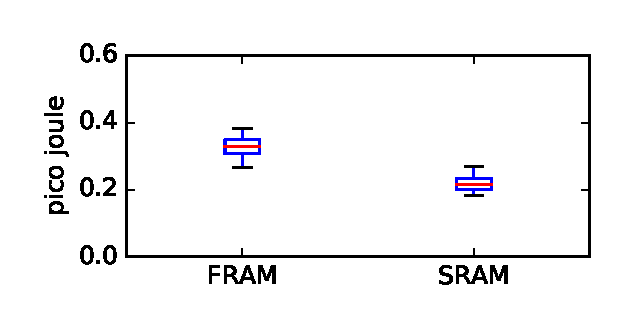
\includegraphics[width=0.49\columnwidth]{figures/fram_write.eps}}
	\subfloat[Energy cost of \emph{read} operation]{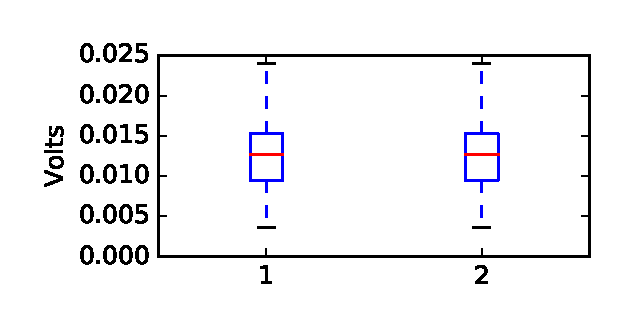
\includegraphics[width=0.49\columnwidth]{figures/fram_read.eps}}
	\caption{Energy cost of accessing volatile (SRAM)/non-volatile (FRAM) memory during write (left) and read (right) operation.}
	\label{fig:framEnergy}
\end{figure}

We have executed an experiment to measure the cost of read/write operations of $w$ to volatile and non-volatile memory. The result is given in Figure~\ref{fig:framEnergy}. Four applications were developed that \emph{access} the FRAM and SRAM of the MSP430FR5969 microcontroller~\cite{msp430datasheet}. The interference free debugger (EDB)~\cite{edb} is used as the energy measurement tool. The EDB probes the energy buffer before and after accessing the FRAM/SRAM 1600 times. This large number of FRAM access is used to increase the reliability of the results generated by the used measurement tool (e.g. reducing the effect of the quantization error). The energy buffer is charged, using the EDB, to $\approx$ 2.45\,V \textbf{only} at the beginning of the execution and of the programs. The write operations were performed by writing literal values, random numbers, to the memory. However, a read operation must be followed by a write operation. Therefore, we chose to write a read value to SRAM. Based on our measurements we conclude that a FRAM access equals $\frac{3}{2}$ SRAM access~\footnote{We remark that TI already mentions~\cite{ti_fram_faq} that FRAM write access is more energy expensive than SRAM write access. However, TI does not quantify this energy overhead.}. Therefore, reducing FRAM access is desirable when developing energy limited software solution---\emph{which is in sharp contrast to the main goal of all checkpoining solutions}.

The above result reassures the intuitive observation that a decrease of CP (Table~\ref{table:chechpoint_comparison}) decreases the energy cost associated with each state preservation method and reduces operation cost which in most simplistic terms is defined as $\mathcal{O}(\text{CP})+\mathcal{O}(\text{PL})$, where PL is the cost of program execution without checkpointing. On the other hand, this increases task/checkpoint re-execution time. The ideal solution is a runtime that \emph{adaptively} changes task size during runtime, which however exposes a second problem.

\paragraph{Problem 2---Modular execution models are not adaptive}

A modular intermittent execution model completely depends on a programmer's estimation which mostly results in a sub-optimal code division. Moreover, this model can only consider a single hardware configuration and it does not take environment variability into considerations. Each battery-less platform has different storage sizes, refer to Table~\ref{table:capacitor}, which causes different charge/discharge periods. This result in different execution times. In the worst case the size of the capacitor might be too small to execute one task written by the programmer. This calls for the ability of the modular execution runtimes to \textbf{merge} multiple small tasks into a larger one or \textbf{split} a large task into a set of small ones on the fly (post-compilation time). Unfortunately the following features prevent us to perform this task using existing runtimes~\cite{chain,alpaca}.

\begin{figure}
	\centering
	%\includegraphics[width=\columnwidth]{figures/Dynamic_chain_sequence_example}
	\caption{Dynamic task merging problem.\todo{Draw merging diagram}{Przemek/Amjad}}
	\label{fig:DynamicChainSeq}
\end{figure}

\begin{itemize}
	\item \textbf{Irreversible tasks transitions} According to both Chain~\cite{chain} and Alpaca~\cite{alpaca} programming models, each task calls the next one. The transition is done through functions calls and manually clearing the stack to prevent the stack overflow problem. This approach makes all the task transitions firm, preventing task merging.

	\item \textbf{Dependency on privatization} Alpaca~\cite{alpaca} extended Chain~\cite{chain} with a concept of privatization, i.e. it protects task-shared variables from WAR dependency problem \emph{within} the scope of a task. Therefore, if tasks are on-demand merged, the scope of these dependencies are changed and the static analysis to privatize these variables is not valid any more and the data consistency can not be preserved.

	\item \textbf{`All channels' requirement} Fig.~\ref{fig:DynamicChainSeq} shows that if the task control flow is a circular with no branches then task merging is possible. Moreover, all the intra-merged-tasks channel can be committed to SRAM instead of FRAM to save energy. However, this execution path is only a special one. If the general case (see again Fig.~\ref{fig:DynamicChainSeq}) is considered then leaving out the intra-merged-task channels might result in data inconsistency. Than is, if an application tries to access a merged task from the middle after a power interrupt then the input for that task is not ready, which result in an incorrect execution.
	
	\item \textbf{Lack of multi-versioning system} All known modular execution models define its own input for each task that is not shared with other tasks. This design decision makes the benefit of merging tasks of less importance since each task is interacting with its own variables. \todo{Rewrite this paragraph: still unclear}{Przemek}
\end{itemize}

\subsection{Main Idea: Tasks Coalescing}

To combat the above limitations we propose a new concept of \textbf{virtualization}: a modular execution model with softening a number of transitions, by keeping the state of the execution progress in the volatile memory, to construct a bigger \emph{virtual task} to reduce energy consumption. Ideally, the size of the virtual task should match the length of a continuous interval of the intermittent power supply for the best performance. Another form of virtualization can be achieved by reducing the number of non-volatile memory accesses. This can be done by having a temporary copy of a global variable in the volatile memory (similar to the caching principle) and a task interacts with it and updates it before writing back the most recent value to the non-volatile memory during the commit process.

\subsection{Assumption on the Type of Computing Hardware}
\label{sec:background_hardware}

Before proceeding further with the background we need to make certain assumptions about the underlying hardware. We assume that we operate on the microcontroller (more generally, computing hardware) equipped with a mix of volatile and non-volatile memory, such as FLASH, Ferroelectric RAM or Magnetoresistive RAM. We do not assume to rely on specific memory type (either volatile or non-volatile), in contrary to earlier works targeting non-volatile processors~\cite{su_date_2017,ratchet,quickrecall,nvp}. Actually, we will exploit the properties of both memory types to maximize performance metrics of the program being executed. We enable to I/O operations, however we do not enable the scheduling of operations (which \emph{nota bene} forms a foundation for a simple runtime). All in all, our hardware model follows in assumptions the two most relevant intermittently-powered execution environments~\cite{alpaca,chain}. \todo{Verify if this section is not out of place}{Brandon}

\subsection{Structuring a Task-based Intermittent Computing Program}

\todo{Please check this is the right way for this section: it reads as it should be in Section 3 describing \sys}{Brandon} Task is a programmer (or compiler) defined code that is executed based on consistent set of inputs, i.e. memory fetched from a specified memory location, producing a consistent output stored in a specified (the same or different) memory location. Syntactically, we can treat a task as a continuous sub-section of a large program encapsulated by (i) task specific keywords defining the beginning and the end of a task and (ii) message passing between tasks connected with each other.

\begin{figure}
	\centering
	%\includegraphics[width=\columnwidth]{figures/taskification_example}
	\caption{Task flow example executed by \sys.\todo{Draw an example task diagram}{Przemek}}
	\label{fig:task_flow_example}
\end{figure}

Let us look into how task-based programming is performed relying on an example provided in Fig.~\ref{fig:task_flow_example}. Each task is uniquely identified by a keyword. A separate part of code specifies a state machine than governs how tasks are connected with each other. This way a programmer specifies to which other task a current task needs to pass the result of its computation (and it can be either a new task or the task itself). Tasks are executed atomically. That is, task will be executed only once and will be considered as completed only when a task reaches a final instruction line informing a scheduler that a program is ready to enter into a new task.

Just like Chain~\cite{chain} and Alpaca~\cite{alpaca}, \sys does not support concurrent programming, multi-threading (multi-task sequence) and does not consider priorities and on-demand scheduling. These features are extremely important to consider but go beyond the scope of this work. A comparative description of \sys is given in Table~\ref{table:feature_comparison}. \todo{Decide if we need such table}{Brandon}

Important and a strong assumption about task-based programming for intermittently-powered systems is that an energy availability for the largest possible task execution must be guaranteed. Task is an atomic operation and must preserve execution order and memory manipulations. Task that follows such an assumption is equivalent to task being executed on a continuously-powered non-interrupted system. Whenever a task cannot fit into a single energy reservoir, it must be divided into tasks that will be executed within a single discharge cycle.

\begin{table}
	\centering
	\footnotesize
	\begin{tabular}{|c|c|c|c|}
		\hline
		{~} & Alpaca~\cite{alpaca} & Chain~\cite{chain} & This work \\
		\hline\hline
		Task connections & in-task & in-task & outside \\
		Task re-use & N & N & Y\\
		Memory model & globals & globals & globals\\
		Concurrency & N & N & N \\
		Task blocking & N & N & Y \\
		Energy-adaptive & N & N & Y \\
		\hline
	\end{tabular}
	\caption{Comparison of existing task-based execution models against \sys.}
	\label{table:feature_comparison}
\end{table}

\todo{Elaborate on the ``key challenge'' paragraphs near the end of the intro}{Przemek}

%We can write the problem of maximizing all task sizes formally as
%
%\begin{equation}
%\underset{i}{\arg\,\max} \sum_{i}m_i+t_i \text{~subject to~} \forall_i mi+t_i>e,
%\end{equation}
%
%where $e$ is the required minimum energy to perform a task, $i$ is the total number of tasks, $m_i$ and $t_i$ are the cost of task traversal (memory copying time of task variables) and time to complete one task, respectively.

%Two problems with fixed-size task in intermittent execution. (a) task underestimation: task executed at device with capacitor size $X$, will not execute at device with capacitor $X\gg Y$; (b) task overestimation: with stable energy source task tracking causes unnecessary overhead.

%\begin{figure}
%\centering
%\includegraphics[width=\columnwidth]{figures/taskification_example}
%\caption{Program divided into tasks.}
%\label{fig:taskification_example}
%\end{figure}

%Other forms of intermittent platforms will share the same problem. One of them considers actuation platforms, which will be powered directly from energy harvesting sources~\cite{}. will share the energy storage with computing platform. However, power supply for actuators is order of magnitude larger than for computation. Therefore, although capacitor is large enough to perform computation alone, energy to power actuators takes precedence leaving not much space for computing.


\section{\sys System Overview}
\label{sec:systemdescription}

\begin{figure}
	\centering
	\includegraphics[width=\columnwidth]{figures/overview.pdf}
	\caption{System's top-level view. \sys is composed of two core components: \emph{Adaptive Task Scheduler} and \emph{Virtual Memory Manager}.}
	\label{fig:system_overview}
\end{figure}
%
\sys is a new programming and execution model for intermittent computing on energy-harvesting devices. \sys addresses the challenges outlined in Section~\ref{sec:background} to make task-based intermittent programs {\em programmable} and {\em efficient}. \sys accomplishes this goal with a constellation of a new programming model and runtime software system support, that supports dynamically adaptive task-based execution. Figure~\ref{fig:system_overview} shows an overview of \sys.

\textbf{Programming and Execution Model.}  To use \sys, a programmer must convert a plain C code into tasks by encapsulating the code in a top-level set of functions, sequences the control-flow between these tasks, and annotates memory accesses that manipulate global data.
The programmer compiles their task-based code, and links to \sys runtime,
producing a \sys-enabled binary. The runtime library relies on \sys's novel
{\em virtual memory manager} and its {\em adaptive task scheduler} to adapt its execution with the energy conditions.

\textbf{Adaptive Task Scheduler.} 
\sys's adaptive task scheduler makes \emph{energy-aware} scheduling decisions to group tasks together or split a task. By coalescing tasks \sys amortizes commit and transition costs, and by a task splitting, after repeated failures on a single task, it avoids the task non-termination problem. The scheduler uses its recent execution history---no hardware dependency---as a metric to estimate energy availability and eventually to decide on the dynamic task size. 

% HERE -----------------------------
\textbf{Virtual Memory Manager.} \sys is able to efficiently coalesce
tasks because of its efficient virtual memory manager. \sys's memory manager
paginates memory and ensures that data in a page remain consistent despite
power interruptions. \sys allows a task to manipulate data in a volatile copy
of a page only. Pages swap between volatile and non-volatile memory, depending
on the capacity of the volatile memory and the program's access pattern. \sys
tracks a task's memory accesses efficiently at page granularity (rather than
using, e.g., costly word-granular tracking). When a task ends, each page it
accessed commits from volatile memory (or from a non-volatile swap region for
dirty pages) back to the non-volatile main memory. Pages efficiently,
atomically commit using a two-phase commit procedure accelerated using hardware
support for direct memory access (DMA). Section~\ref{sec:memory_virtulaization}
provides details of \sys's memory manager.

\section{\sys Task Adaptation}
\label{sec:task_adaptation}

\sys is able to virtually merge tasks to construct a bigger virtual task and commit the state of the virtual task instead of the individual real tasks. 

\subsubsection{Task Merging Algorithms}



\subsubsection{Power Interrupt Immune Scheduler}

% TNT :  Total Number of Tasks
% JT 	: Total Jump
% ID	: Task ID
% D	: relative Jump (Delta)
% VCT_PT : Current Task Pointer

% if(TJ < TNT)
% 	VCT_PT <- VCT_PT + D
% else
% 	while ((dis = TJ - TNT) > TNT)
% 		dis -= ID
% 	VCT_PT <- VCT_PT + dis


\begin{algorithm}[t]
	\caption{\sys's scheduler: relative jump algorithm}
	\label{algo:relativeJump}
	\scriptsize
	%\small
	\begin{algorithmic}[1]
			\State \textsf{TNT}: Total Number of Tasks
			\State \textsf{ID}: Task ID
			\State \textsf{$\delta$}: Relative Jump
			\State $\textsf{TJ} \leftarrow (\textsf{ID} + \delta )$ \Comment{Total Jump}
			\State \textsf{\textsf{$VCT_{pt}$}}: Virtual Current Task Pointer

			\If { \textsf{TJ} > \textsf{TNT} }
				\State $\textsf{dis} = \textsf{TJ} - \textsf{TNT}$
				\While{ $ \textsf{dis} > TNT $ }
					\State $\textsf{dis} -= \textsf{TNT}$
				\EndWhile
				\State $\textsf{dis} -= \textsf{ID}$
				\State \textsf{$VCT_{pt}$} $+= \textsf{dis}$
			\Else
				\State \textsf{$VCT_{pt}$} $+= \delta $

			\EndIf
	\end{algorithmic}
\end{algorithm} %Task jumping algorithm

It utilizes a persistent circular buffer (persistent linked list) to keep the state of a program across power failures. \sys provides an API to enable a programmer to have a full control over the execution flow of the program, i.e. (un)blocking a task or re-execute the same task which is particularly important in the intermittent execution to emulate a persistent loop. 

\paragraph{Fixed Virtual Task Size}

	\begin{algorithm}
		\caption{Task coalescing mechanism}
		\label{algo:fixVirtTask}
		\scriptsize
		%\small
		\begin{algorithmic}[1]
			\State $VT \subset \text{\{\sys Tasks\}} $  \Comment{$VT:$ Virtual Task}
			\State VTS : VT size
			\State MVTS: maximum VT size \Comment{line added in fixed size approach}
			\vspace{0.1cm}

			\While {$True$}
				\State $VT \leftarrow VT_{next}$
				\vspace{0.1cm}
				\While {execute $VT$} 
					\If { $\text{power failed twice}$ }				
							\State $VTS--$  
							\State $ MVTS = VTS $ \Comment{line added in fixed size approach}
						\EndIf
				\EndWhile

				\vspace{0.1cm}
				\If {$ \text{All tasks executed}$}
					\If{$VTS < MVTS$} \Comment{line added in fixed size approach}
					\State $VTS++$
					\EndIf
				\EndIf
			\EndWhile
		\end{algorithmic}
	\end{algorithm}

\begin{figure}
	\centering
	\includegraphics[width=0.8\columnwidth]{figures/virtualTaskSize.eps}
	\caption{Size of the virtual task versus the execution time of a dummy application that contains 12 empty tasks.}
	\label{fig:virtualTaskSize}
\end{figure}

\begin{figure}
	\centering
	%\includegraphics[width=0.25\columnwidth]{figures/task_coalescing}
	\caption{Task coalescing architecture.}
	\label{fig:}
\end{figure}

The question remains, is the best strategy to coalesce all tasks into a singe one, as the energy becomes fully available, i.e. from energy harvesting to continuous power environment. To answer this question we have implemented a simple program composed of $x$ empty tasks.  Figure~\ref{fig:virtualTaskSize} shows the benefit of virtualizing the Modular Intermittent Execution Mode (MIEM) in the best case scenario (continuous power supply). 


%\begin{algorithm}
%	\caption{Opportunistic virtual Task size}
%	\label{algo:fixVirtTask}
%	\scriptsize
%	%\small
%	\begin{algorithmic}[1]
%		\State $VT \subset \text{\{\sys Tasks\}} $  \Comment{$VT:$ Virtual Task}
%		\State VTS : VT size
%		\vspace{0.1cm}
%		
%		\While {$True$}
%		\State $VT \leftarrow VT_{next}$
%		\vspace{0.1cm}
%		\While {execute $VT$} 
%		\If { $\text{power failed twice}$ }				
%		\State $VTS--$  
%		\EndIf
%		\EndWhile
%		
%		\vspace{0.1cm}
%		\If {$ \text{All tasks executed}$}
%		\State $VTS++$
%		\EndIf
%		\EndWhile
%	\end{algorithmic}
%\end{algorithm}
\subsection{Task Downsizing}
\label{sec:task_downsizing}

We proceed with the second task adaptation feature of \sys, namely reduction of the task size boundary to enable execution of a program on any energy buffer size.

\begin{figure}
	\caption{\todo{Figure to describe partial commit is needed}{Sinan, Carlo}}
\end{figure}

\subsubsection{When Task Downsizing is Triggered}

If power fails consecutively twice before the system can complete one single static task, it means that the static task requires more energy than currently available in a discharge cycle, so it is necessary to have a mechanism to execute a chunk of the task, save the partial progress through the task, and continue try to run the rest of the task. If a power failure occurs after saving partial task progress, the system makes forward progress, albeit without task atomicity. \sys may save partial task progress multiple times before completing a very long task. To avoid the fail-stop case of non-termination, \sys's partial commit mechanism will split tasks that have not been marked as atomic by the programmer.

A partial commit saves the stack, registers and the volatile pages to the non-volatile memory. \sys starts with a big random guess and down-scales it using a binary search until it succeeds in preserving the partial execution progress. The obtained value is the initial seed for the next partial commit procedure.

\textcolor{red}{More variables describing the partial commit algorithm: we do not explore as many options for partial commit as we do for coalescing}

\todo{Proof of the maximum granularity of task downscaling - show it is limited by the clock}{Carlo}

\subsubsection{Why Task Downsizing is not \sys's Default Behavior}

Task downsizing is the core novelty of \sys when it comes to code portability and re-usability. However, it has limitations, which force  it to be a non-default \sys behavior. 

\textbf{Static deployment of partial commit stubs.} This approach reduces programmer effort, although the programmer still needs to apply \sys's API and distribute trigger points for partial commits. On the other hand, \sys' downsizing introduces an additional overhead by saving the stack and the register file each time it commits the pages. 

\textbf{Dynamic deployment of partial commit stubs.} \sys downsizing does not rely on any information from the programmer to trigger the commit process. However, \sys utilizes a trial and error approach to optimize the commit rate over the entire program execution time. Therefore, it suffers from a large cumulative re-execution penalty.

\section{\sys Memory Management}
\label{sec:memory_virtulaization}

One of the main objectives of \sys run-time is to restrict tasks to interface only with the volatile memory, since volatile memory access is relatively cheaper, as we already have shown experimentally in Section~\ref{section:background_task_computing} (Problem 1, Figure~\ref{fig:framEnergy}). This feature will also provide several advantages during task coalescing, as we will be dealing with in Section \ref{sec:task_coalescing}.

\subsection{Intermittent Volatile-Only Memory Access}
\label{sec:virtualization_problems}

In order to enable volatile-only memory access, the persistent variables a task operates on should be brought from non-volatile memory to a fixed-sized \emph{volatile buffer} in the main memory. During its execution, the active task reads and modifies only the contents of this buffer. When the task is finished its execution, the modified variables, i.e. memory locations, in this buffer should be committed back to their original locations in non-volatile memory. We list three fundamental problems proving that this is however a non-trivial task. 

\begin{figure}[t]
	\centering
	\includegraphics[width=\columnwidth]{figures/sram-buffer}
	\caption{The interaction between the task, volatile buffer and the non-volatile memory (FRAM). Initially, the persistent variable \texttt{x} is not in the volatile buffer but \texttt{y} and \texttt{z} are.}
	\label{fig:volatile-buffer}
\end{figure}

\paragraph{Problem 1---Runtime Access Overhead:} The persistent variables read and/or modified by a task might not be known in advance due to the dynamic program flow. Therefore, the volatile buffer should keep track of the persistent variables at runtime, as presented in Figure~\ref{fig:volatile-buffer}. When a persistent variable is read or written (refer to steps 1 and 3--5 in Figure~\ref{fig:volatile-buffer}) first the volatile copy of the corresponding variable is \emph{searched} in this buffer. If it is found, the read or write operation is performed on the volatile copy. Otherwise, the persistent variable is read from the non-volatile memory and inserted in this buffer for future operations (refer step 2 in Figure~\ref{fig:volatile-buffer}). Unfortunately, we observed that \emph{search--bring} operations at each access to the persistent variables introduce considerable overhead (refer to Figure~\ref{fig:dmaTimeEnergy} and pointer-based operation therein) and might nullify the benefit of task coalescing, a cores \sys feature.

\begin{figure}[t]
	\centering
	\subfloat[Time needed to transfer a block of data]{\includegraphics[width=0.49\columnwidth]{figures/dmaSize_time.eps} }
	\subfloat[Energy needed to transfer a block of data]{\includegraphics[width=0.49\columnwidth]{figures/energyConsumptionDMA_SW.eps}}
	\caption{Time and energy consumption of moving a block of data from SRAM to FRAM: CPU intervention versus Direct Memory Access (DMA).\todo{Explain HW/SW setup; make fonts larger, unify legends and axes}{Amjad}}
	\label{fig:dmaTimeEnergy}
\end{figure}

\paragraph{Problem 2---Two Phase Commit Overhead:} For the consistency of the non-volatile memory, the volatile buffer should be committed at the end of each task by means of a \emph{two-phase commit}---refer Figure~\ref{fig:volatile-buffer} steps 6--8 for the first phase and 9--11 for the second step of the commit operation. However, two-phase commit is also expensive since the committed variables are not \emph{contiguous}---leading the fact that copying or moving of data between/within volatile and non-volatile memory should be always performed selectively with CPU intervention. Non-selective block memory copy operations using Direct Memory Access (DMA) that eliminates CPU intervention are considerably more efficient, refer again to Figure~\ref{fig:dmaTimeEnergy} for a comparison, but infeasible in this case.

\paragraph{Problem 3---Memory Fit Constraints:} Persistent variables can be allocated \emph{contiguously} in non-volatile memory with compiler support. In order to eliminate run-time buffer \emph{search} overhead (by not relying on specialized hardware such as e.g. in~\cite{hicks_isca_2017}), \emph{all} persistent variables can be brought from non-volatile memory to the volatile buffer at system start-up---very efficiently and faster thanks to DMA for \emph{block} memory-memory copy/move operations. Two-phase commit is also very efficient in this case since DMA can be utilized to move volatile buffer as a block to the corresponding non-volatile locations. However, bringing all persistent variables from non-volatile memory to the volatile buffer suffers from the \emph{memory fit problem}: the volatile memory is a scarce resource and may not be large enough to hold all persistent variables.

\subsection{Software-based Paging Mechanism} 

Considering these facts, \sys implements a \emph{paging-based} virtual memory in software that (i) partitions contiguously allocated persistent variables into pages; (ii) implements the volatile \emph{page buffer} that holds a single page; (iii) swaps the page in volatile memory with a new page in non-volatile memory efficiently by utilizing DMA-based memory block-copy operations; (iv) buffers the swapped volatile page until commit to enable task coalescing which we describe in Section~\ref{sec:task_coalescing}; (v) implements two-phase commit of the modified pages to preserve the consistency of non-volatile memory; and (vi) performs this two-phase commit operations using DMA for the sake of efficiency. We now explain the details of \sys paging mechanism.

\subsubsection{Address Translation and Variable Access}

\sys virtual memory system provides an interface to the applications which is composed of two C macros: \texttt{RVAR(var)} and \texttt{WVAR(var,val)} that accept the name of the persistent variable \texttt{var} as an input argument. These macros obtain the \emph{physical address} of the corresponding persistent variable in non-volatile memory and translates it into the \emph{virtual address} in page buffer \texttt{pageBuf} in volatile memory, which is composed of a \emph{page tag} and \emph{offset}. For the sake of simplicity and efficiency, we implemented this translation in a trivial way: the first byte of the physical address is considered to be the page tag and the rest is the offset within the corresponding page. 

\begin{algorithm}[t]
	\caption{\texttt{RVAR(var)} pseudo-code}
	\label{algo:rwar}
	\scriptsize
	%\small
	\begin{algorithmic}[1]
		\State $\texttt{tag}\leftarrow \texttt{getTag(var)}$ 
		\If { \texttt{tag} != \texttt{CrntPagTag} }	\Comment{Check if the page is in the page buffer}
		\State	\texttt{PageFault(tag)} \Comment{Page is not in the page buffer, bring it}
		\EndIf
				\State $\texttt{offset}\leftarrow \texttt{getOffset(var)}$ 		
		\State \texttt{return pageBuf[offset]}  \Comment{Return directly from page buffer}
	\end{algorithmic}
\end{algorithm}

After address translation and obtaining the virtual address, it is required to check if the corresponding page is already in volatile page buffer. \sys maintains a \texttt{CrntPagTag} variable that holds the tag of the page currently in the page buffer. If the tag of the virtual address and \texttt{CrntPagTag} are equal, this indicates that page buffer holds the required page and the offset of the virtual address can be used to read from/write to the location in the volatile page buffer immediately. If the required page is not in the page buffer, a \emph{page fault} routine is executed as we discuss in the section below. Observe that the computational complexity of the whole steps pertaining to address translation and variable access is $\mathcal{O}(1)$---introducing minimal overhead to the system to boost up benefits of volatile-only memory interfacing. The pseudo-code of \texttt{RVAR}, which is quite similar to that of \texttt{WVAR}, is presented in Algorithm~\ref{algo:rwar}.

\subsubsection{Page Faults and Page Swapping}

\begin{algorithm}[t]
	\caption{\texttt{PageFault(tag)} pseudo-code}
	\label{algo:pagefault}
	\scriptsize
	%\small
	\begin{algorithmic}[1]
		\If {\texttt{isDirty(CrntPagTag)} }	\Comment{Check if the active page is modified}
		\State \texttt{pageCommit(pagesTemp)} \Comment{Phase I commit the active page}
		\EndIf
		\If {\texttt{isDirty(tag)}} \Comment{Check if the requested page has been modified}
		\State {\texttt{getPage(tag,pagesTemp)}=false} \Comment{Get page from the temporary buffer}
		\Else
		\State \texttt{getPage(tag,pagesOrg)}=false \Comment{Get page from the original location}
		\EndIf 
		\State \texttt{CrntPagTag} = \texttt{tag} \Comment{Update tag}
	\end{algorithmic}
\end{algorithm}

If the page tag of the variable \texttt{var} and \texttt{CrntPagTag} are not equal (e.g. Lines 2--3 of Algorithm\,\ref{algo:rwar}), the active page, i.e. the contents of the page buffer \texttt{pageBuf}, should be swapped with the page whose tag is equal to the \texttt{var}'s tag. The pseudo-code of the Algorithm \texttt{PageFault} that handles this operation is presented in Algorithm~\ref{algo:pagefault}. This algorithm handles two fundamental cases.

\paragraph{Case 1---Modified Active Page:} If the task performed at least \texttt{WVAR} operation, then the page buffer \texttt{pageBuf} that holds the current active page is modified (Line 1 of Algorithm~\ref{algo:pagefault}). In order to keep the modified values of the variables, the active page is committed to an intermediate page buffer in non-volatile memory, namely to \texttt{pagesTemp}. This operation can be considered as first phase of the commit operation, as we present in the next section. If the active page is not modified, there is no need to commit it to the temporary page buffer.

\paragraph{Case 2---Modified Requested Page:} After committing the active page to its temporary location, Algorithm~\ref{algo:pagefault} checks if the requested page is modified previously by the same task (Line 3). If this is the case, the requested page should be be brought from \texttt{pagesTemp} rather than its original location in non-volatile memory (Line 4), so that the task accesses the modified values of the persistent variables. Otherwise, the requested page is brought from its original location, i.e. \texttt{pagesOrg} (Line 6). After the swapping operation, the \texttt{CrntPagTag} is set to the tag of the requested page (Line 7). It should be noted that DMA is used to memory block copy operations, introducing minimal overhead during page swapping. 

\subsubsection{Pages Final Committing}

After a task finishes its execution, all pages committed to \texttt{pagesTemp} should be committed to their original locations in \texttt{pagesOrg}. This is the second phase of the \emph{two-phase commit} operation. As mentioned previously, memory block copy operations for the second phase commit is also utilized by DMA.

\subsection{Non-Volatile Memory Consistency Issues}

During the execution of any task, modifications to the persistent variables will not be reflected to the original locations in the non-volatile memory, since the task interfaces with only the volatile page buffer \texttt{pageBuf} and the modifications are temporarily stored in the non-volatile \texttt{pagesTemp} buffer. The changes stored in the \texttt{pagesTmp} is committed to the original locations in \texttt{pagesOrg} after the task is finished its execution. Therefore, any power interruptions within the execution will not lead to inconsistencies in the \texttt{pagesOrg} when the task is re-executed after a power boot. As a consequence, the proposed paging mechanism keeps the consistency of the non-volatile memory thanks to the two-phase commit operation for the modified pages. 

%\todo{Benefits of the paging to the task coalescing should be mentioned in the next section}{Amjad/Przemek/Sinan}

\section{\sys Implementation}
\label{sec:implementation}

We proceed with the explanation of the implementation of \sys programming model. \sys implementation is light and adds very little on top of a plain C language.

\subsection{\sys Application Programming Interface}
\label{sec:coala_api}

Coala's API adds only five syntactic constructs to a C-based language: (i) \texttt{COALA\_TASK}: declaration of a new task, (ii) \texttt{COALA\_NEXT\_TASK}: declaration of the next task to be scheduled after the currently executing one completes, (iii) \texttt{COALA\_PV}: declaration of a new protected variable, (iv) \texttt{RP}: declaration of a protected variable read, and (v) \texttt{WP}: declaration of a protected variable write. Moreover, the programmer is required to explicitly call two \sys API functions inside the main program body: (i) \texttt{COALA\_INIT}: to pass as an argument the global initialization task to run upon the first boot , and (ii) \texttt{COALA\_RUN}: which hands the control to \sys's scheduler. Finally, when the programmer intends to \texttt{typedef} a \texttt{struct} to use it as a protected variable, she/he need to declare each structure's member by using the \texttt{COALA\_SM} macro to ensure proper memory alignment required by \sys's page handler.

Table~\ref{table:coala_api} summarizes \sys's API methods and their arguments. \todo{Add example of a Coala program}{Carlo, Przemek} These methods trigger specific \sys kernel functions, whose explanation is given in the following sections.

\begin{table}
\centering
\begin{tabular}{| r | p{0.7\columnwidth} |}
	\hline
	{Method} & {Arguments} \\
	\hline\hline
	\texttt{COALA\_INIT}(t) & $t \in \mathbf{T}$: task to be scheduled on a first boot \\
	\hline
	\texttt{COALA\_RUN}() & --- \\
	\hline
	\texttt{COALA\_TASK}($t$, $w_t$) & $t \in \mathbf{T}$: new task name, $w_t$: weight of task $t$ \\
	\hline
	\texttt{COALA\_NEXT\_TASK}($t$) & $t \in \mathbf{T}$ : next task to be scheduled\\
	\hline
	\texttt{COALA\_PV}($p$, $v$ [, $s$]) & $p$: variable type, $v \in \mathbf{V}$: new protected variable name, $s$: array size\\
	\hline
	$u$ := \texttt{RP}($v$) & $v \in \mathbf{V}$: protected variable to be read, $u$: value \\
	\hline	
	\texttt{WP}($v$) := $u$ &  $v \in \mathbf{V}$: protected variable to be written, $u$: value \\
	\hline
	\texttt{COALA\_SM}($p$, $m$ [, $s$]) & $p$: \texttt{struct} member's type, $m$: \texttt{struct} member's name, $s$: array size \\
	\hline
\end{tabular}
\caption{Summary of \sys API; $\mathbf{T}$: set of all tasks, $\mathbf{V}$: set of all protected variables, $[, s]$: optional argument.}
\label{table:coala_api}
\end{table}

\subsection{\sys Kernel Functions Implementation}

\textbf{New Tasks.} The API method \texttt{COALA\_TASK} statically allocates a non-volatile constant variable holding the task weight, and declares a void function with the name passed as an argument.

\textbf{New Protected Variables.} The API method \texttt{COALA\_PV} statically allocates (and aligns in memory) a non-volatile variable, whose address will be used by \texttt{RP} and \texttt{WP} API methods to locate the most recent location of the variable itself, which could be either the location of the variable in volatile memory or its location in a non-volatile memory.

\textbf{Task Transitions.} By calling \texttt{COALA\_NEXT\_TASK} API method, the programmer tells \sys's scheduler what task to execute next. The \sys kernel implementation is built on the assumption that the currently executing task is not interrupted, and only once it completes the next task is run. \todo{Provide information on the implementation - this paragraph repeats simply what previous section did}{Carlo}

\textbf{Protected Reads and Writes.} When \texttt{RP} and \texttt{WP} API mentods are used, \sys searches the volatile memory for the page the protected variable belongs to. If such page is not found in RAM, then a page fault occurs, and the page is fetched from the non-volatile memory. The two functions return a handle to the variable's volatile memory location. Unlike \texttt{RP}, \texttt{WP} marks the page being written as dirty, so that it can be committed to its non-volatile location.

\textbf{Initialization and Origin Task.} The behavior of the API method \texttt{COALA\_INIT} is very similar to \texttt{COALA\_NEXT\_TASK}, with the addition that all the preliminary kernel initializations are performed inside this function. Moreover, the origin task is scheduled only upon the first boot.

\begin{wrapfigure}{t!}{0.5\textwidth}
	\centering
	%\includegraphics[width=0.5\columnwidth]{figures/graffle/overview.pdf}
	\caption{\sys state machine implementation \todo{Draw a figure}{Sinan, Carlo}}
	\label{fig:coala_state_machine}
\end{wrapfigure}

\textbf{Execution.} The application control is passed to \sys's scheduler by calling \texttt{COALA\_RUN} at the end of the main function. A high-level state machine of the scheduler is depicted in Figure~\ref{fig:coala_state_machine} \todo{Draw a figure; provide more text on the execution}{Carlo}.

\subsection{\sys Paging Implementation}

\textcolor{red}{THIS IS UNEDITED AND SHOULD NOT BE READ YET - Placeholder}

Memory virtualization. Working (volatile) buffer, store and shadow (non-volatile) buffers. No major changes since last version.

Page allocation and page tags. When the application accesses a protected variable with RP or WP, Coala has to search for the variable in RAM first, and in non-volatile memory if it not found in RAM. Actually, the kernel searches for pages, not single variables. A page search can be very fast if each page is identified by a unique tag, and if every variable belonging to a page bears the tag in its address. Thus, retrieving a page tag from a protected variable’s address boils down to extracting the upper bits of the address itself. The remaining lower bits denote the variable’s offset in its page.

\begin{figure}
	\centering
	\includegraphics[width=\textwidth]{figures/graffle/paging.pdf}
	\caption{Illustration of \sys page tags.}
\end{figure}

In order to obtain unique page tags, some alignment requirements have to be met. First, the page size $S$ has to be a power of two. Moreover, pages in non-volatile memory have to be aligned by $S$. In the example above, $S$ is 256, and every page’s first address is a multiple of 256. Note that, by aligning pages by $2n$, the alignment is also valid for all sizes $2^x$ with $x \leq n$.

Page fault and page swap (with DMA). When a page is not found in RAM, it is fetched from FRAM. No major changes since last version.

\subsection{\sys Scheduling and Committing}

Target budget initialization. Upon a reboot, the target budget (or target coalesced task size) has to be updated depending on the coalescing strategy [...].

Coalescing state recall. The last (coalesced) task has to be recalled. More specifically, the function pointer of the last coalesced task has to be retrieved from NV memory, where is had been saved during the last successful commit. [...].

Partial execution restoration. In case there is a valid partial execution checkpoint, the program has to resume from there [...].

Coalesced scheduling. Static tasks are coalesced and run [...].

Intermediate commit and ultimate commit. When a coalesced task is successfully run to completion, all the dirty pages in SRAM have to be persistently saved to non-volatile memory. Since last version, no major changes were made to the intermediate commit (SRAM to shadow buffer), but an optimization was applied to the ultimate commit (shadow buffer to store buffer). Store buffer and shadow buffer used to be physically separated in memory. Now, the role of a block of memory (i.e. a page) is interchangeable, meaning that, during the ultimate commit, the shadow buffer pages that were written during the previous commit phase become store buffer pages, and their relative store buffer pages become shadow buffer pages. A page’s role is retrieved using an indirection table, i.e. an array that holds a zero for all the pages whose store buffer resides in the lower memory block, and a one for all the pages whose store buffer is located in the upper memory block. This allows for a lighter commit process, since fewer page moves are performed.

\begin{figure}
	\caption{Intermediate commit and ultimate commit Illustration \textcolor{red}{to be drawn}}
\end{figure}

Target budget update. Before starting a new coalesced task, the target budget (or target coalesced task size) has to be updated depending on the coalescing strategy [...].

\textcolor{red}{API of the partial commit needs to be explained as well}

%\section{Discussion}
%\label{sec:discussion}

%\subsection{Task Coalescing}
\label{sec:discussion_coalescing}

We speculate that a non-obvious benefit of task coalescing is a secure computation support. That is, if the size of the virtual task increases infinitely, it will eventually exceed the maximum size allowed by the energy reservoir. Therefore the program will never finish executing the virtual task. Unless the intermittently-powered device will be physically close to the harvestable energy source and charging rate is larger than the discharging rate, the computation will never complete. This way we entangle \emph{physical proximity} of the device with \emph{success rate} of the computation.

\section{Methodology}
\label{sec:methodology}

Our hardware and software suite used to evaluate \sys novel intermittent execution model represents the  real implementation of low-power intermittent system. As our implementation makes no system assumptions (we execute \sys model on a \emph{real} hardware powered by \emph{real} intermittent source), therefore promises to generate the ultimate set of \sys performance metrics. 

\subsection{Intermittent Platform and Hardware Toolchain}
\label{sec:results_hardware_software}

We evaluated \sys in two power supply environments: (i)  \emph{intermittent} and (ii) \emph{fixed} (to benchmark the intermittent power supply results). In the experiments with intermittent power supply, we evaluated \sys using a WISP\,5.1~\cite{wisp5,wisp}---energy-harvesting platform build around a MSP430FR5969~\cite{wolverine} MCU with 64\,kB of FRAM. We powered the WISP using RF signal generator~\cite{} \todo{Add reference to signal generator}{Przemek} emitting 20\,dBm sinusoidal wave at 915\,MHz.  Signal generator was connected to the Liard RFMAX S9028PCRJ 8\,dBic antenna~\cite{atlas2015}. For distance-controlled experiments, we affixed WISP at two paper protrusions around 10\,cm from the surface of the table (parallel to, and at the edge of, table surface). Antenna of the signal generator was facing WISP directly and located at three distances, $d=\{15, 30, 50\}$\,cm, from WISP. For task coalescing experiments, an additional distance of $d=60$\,cm was considered. Both antennas were parallel to each other and no physical objects were located between the WISP and signal generator antenna. For continuous power experiments we used an alternative setup with MSP-EXP430FR5969 launchpad~\cite{MSP-EXP430FR5969_launchpad}, which had the same MCU as WISP. In all the experiments the timing measurements were performed using either the Saleae~\cite{saleae} logic analyzer (for intermittent power experiments) or TI Code Composer Studio (for fixed power experiments). Both type of experiments are explained in the following section.

\subsection{Software Benchmarks}
\label{sec:software_benchmarks}

\begin{table}
	\centering
	\footnotesize
	\begin{tabular}{| r | p{0.85\columnwidth} |}
		\hline
		Application & Description \\
		\hline\hline
		\textbf{ar} & nearest neighbor classification of randomly generated data modeling a three-axis accelerometer\\
		\hline
		\textbf{bc} & counts bits in byte pseudo-random string using several algorithms, and compares results for correctness\\
		\hline
		\textbf{cuckoo} & Bloom-filter-like Cuckoo filter: first hashes a sequence of pseudo-random numbers, then queries the filter to recover the sequence\\
		\hline
		\textbf{dijkstra} &  Dijkstra algorithm executed continously on a predefined adjecency matrix\\
		\hline
		\textbf{fft} & continuously repeating Fast Fourier Transform on three pre-generated 128 sample vector\\
		\hline
		\textbf{sort} & selection sort algorithm on a fixed sequence of numbers\\
		\hline
	\end{tabular}
\caption{Suite of benchmark applications used in evaluating \sys performance. All applications have been chosen from MiBench testing suite~\cite{mibench,hicks_mibench2_2016}.\todo{Consider adding more information here}{Brandon}}
\label{table:benchmark_table}
\end{table}

We evaluated \sys using benchmarks that originate from the MiBench testing suite~\cite{mibench,hicks_mibench2_2016}. Set of implemented benchmarks is presented in Table~\ref{table:benchmark_table} and their implementation is available via~\cite{coala_website}. Three benchmarks (\textbf{ar}, \textbf{bc}, \textbf{cuckoo}) were implemented by Chain~\cite{chain} and Alpaca~\cite{alpaca}. Three remaining ones (\textbf{dijkstra}, \textbf{fft}, \textbf{sort}) are added as new. \todo{justify the selection of these benchmarks}{Przemek, Carlo, Amjad, Brandon}

%Specifically, we have implemented three benchmarks used by Chain~\cite{chain} and Alpaca~\cite{alpaca} (source code is accessible~\cite{coala_website}), namely: \textbf{ar}: nearest neighbor classification of randomly generated data modeling a three-axis accelerometer; \textbf{bc}: counts bits in byte pseudo-random string using several algorithms, and compares results for correctness; \textbf{cuckoo}: Bloom-filter-like Cuckoo filter that first hashes a sequence of pseudo-random numbers, then queries the filter to recover the sequence. Additionally, we have ported three new benchmarks from~\cite{mibench}, namely: \textbf{dijkstra}: Dijkstra algorithm executed continously on a predefined adjecency matrix; \textbf{fft}: continuously repeating Fast Fourier Transform on three pre-generated 128 sample vector; and \textbf{sort}: selection sort algorithm on a fixed sequence of numbers. \todo{justify the selection of these benchmarks}

All applications were compiled using GCC version 3.8.0. \todo{Check if this still holds}{Przemek} We compare \sys against state-of-the-art task-based runtime Alpaca~\cite{alpaca}. We do not compare \sys against Chain~\cite{chain}, another task-based system, which is inferior to Alpaca in its performance. Also, we do not compare \sys to checkpointing-based systems, such as DINO~\cite{dino} or Mementos~\cite{mementos} (cf. Section~\ref{sec:background_consistency}), as both of them are build on top LLVM compiler, which performance is inferior to GCC compiler used in the evaluation of \sys \todo{Please check if the LLVM compiler argument makes sense}{Brandon}.

\section{\sys Evaluation}
\label{sec:evaluation}

We compare the performance of \sys against the state-of-the-art intermittent execution approach---Chain~\cite{chain}.

The applications that were used in the evaluation are given in Table~\ref{table:benchmark_list}.

\begin{table}
	\begin{tabular}{|c|c|c|}
		\hline
		Name & SLOC (\sys) & SLOC (Chain~\cite{chain})\\
		\hline\hline
		Temperature sensing & 388 & 721 \\ %53\%
		Cuckoo & 483 & 762 \\ %63\%
		RSA & 887 & 1233 \\ %71\%
		DFT & --- & --- \\ %Two resolutions: 4 and 8 Bytes
		Huffman & --- & --- \\ %Data decompression size: 100 bytes
		Selection sort & --- & --- \\
		\hline
	\end{tabular}
\caption{List of benchmarks used in \sys evaluation.}
\label{table:benchmark_list}
\end{table}

\subsection{Continuous Power Supply}
\label{sec:results_continuous_power}

\begin{figure}
	\centering
	\includegraphics[width=\columnwidth]{figures/chain_vipe}
	\caption{Time to complete for a set of testing applications (refer to Table~\cite{table:benchmark_list}) using \sys versus Chain.}
	\label{fig:IPOSPerformance}
\end{figure}

Fig.~\ref{fig:IPOSPerformance} shows that \sys requires a shorter execution time to execute an application under the modular execution model. The size of the virtual task that \sys uses is one real task, i.e. no task coalescing is applied.

%Set of experiments

%- Compiler result: taskifying completion time, correctness, 
%- Task coalescing experiment: with WISP at 3 distances and with fixed power, for all apps, compared against chain, show amount of task merged, time to completion/inter-operation time, overhead (in terms of what?), energy consumed
%- Battery-less microphone: with \sys and without \sys, compared against Chain, 
%- Paging/memory experiment: ?

\subsection{Intermittent Power Supply}
\label{sec:intermittent_continuous_power}

\section{Related Work}
\label{sec:related_work}

\noindent \textbf{Intermittently-Powered Devices:} There is plentiful of research results available on energy harvesting, or more specifically wireless power provision, for embedded devices like sensors or microcontrollers. This paragraph is too short to cover this area extensively and we refer the reader to overview papers~\cite{prasad_comst_2014,sample_procieee_2013,huang:commag:2015,visser_procieee_2013,kamalinejad_commag_2015,ku_cst_2016} for in-depth discussion. With power consumption of electronics going down dramatically with every year, computing systems can be now powered completely from ambient energy. This opens new research areas such as radio frequency-powered computers~\cite{patel_pervasive_2017,rf_powered_computing_gollakota_2014}. Indeed, plenty of new embedded platforms appear that are powered solely from ambient (intentional or non-intentional) energy and include~\cite{wisp5,moo,zhao_rfid_2015,holleman_biocas_2008,thomas_jbcs_2012,naderiparizi_rfid_2015,rodriguez_tbcs_2015,liu_sigcomm_2013,kicksat,nadeau_naturebio_2017}. But there is a price tag associated to them: harvested energy is miniscule, unstable, difficult to predict ergo \emph{intermittent}. Therefore, to guarantee completion of computing, programming and runtime models are being actively researched that are specifically tailored to these intermittently-powered systems. \todo{Revise this section}{Brandon}

\noindent \textbf{Intermittent Execution Environments:} Earlier work include Dewdrop~\cite{dewdrop} (splitting task such that they fill-in the capacitor). Similar, specific-application tailored system includes Wisent and Stork~\cite{stork,wisent}. Checkpoint runtimes include DINO~\cite{dino}, Quickrecall~\cite{quickrecall}, Hibernus/Hibernus++~\cite{hibernus,hibernusplusplus} are checkpointing-based systems requiring hardware support to measure remaining storage energy---a feature prohibitive given typical high energy cost expenditure of such hardware. The only available Task-based intermittent runtime systems are Chain~\cite{chain} and Alpaca~\cite{alpaca}. \sys goes beyond what any task-based system performed by providing \emph{automatic} task creation and \emph{adaptivity} to energy state and energy storage \emph{obliviousness} of the compiled code. \todo{complete this section}{Przemek}

\noindent \textbf{Memory Virtualization:} Review of memory virtualization environments (not necessarily for intermittent power devices). \todo{Fill-in this section}{Przemek}

\section{Conclusions}
\label{sec:conclusions}

This paper presented \sys: a new task-based runtime for intermittently-powered devices that does not require any hardware support. \sys core new features are: (i)  adaptive task coalescing---enabling fast execution despite changing energy arrivals and enabling re-use of the same code on intermittent systems with varying energy reservoirs, (ii) memory virtualization---improving the execution speeds of broad set of benchmarks executed on popular energy-harvesting embedded platform, and (iii) automatic task-generation---removing programmer from the program re-composition to the intermittent domain \emph{almost completely}. \sys, with its task creation/execution automation, responses to the need that all existing predecessors of \sys advocated.

%We believe that \sys is a next major step in enabling computing community to enter the intermittent-power domain without big learning investments.

%Next step in \sys design is the introduction of features needed to implement first fully-operational operating system for transiently-powered devices.

\bibliographystyle{plain}
\bibliography{bib}

\end{document}
